\chapter{Identyfikacja}


\section{Identyfikacja parametrów śmigieł.}

W celu wyznaczenia dynamiki śmigieł helikoptera odpowiedzialnych za ruch odpowiednio względem osi pionowej - Pitch jak i poziomej - Azimuth, przeanalizowano odpowiedzi obiektu na wymuszenie w postaci skoku jednostkowego. Zmiana prędkości obrotowej każdego ze śmigieł, w reakcji na skokową zmianę napięcia zasilania, posłużyła do wyznaczenia parametrów transmitancji. Na bazie przeprowadzonych doświadczeń przyjęto, że każde ze śmigieł jest obiektem inercyjnym pierwszego rzędu w sytuacji gdy sygnałem wejściowym jest napięcie zasilania, a wyjściowym prędkość obrotowa. Do wyznaczenia parametrów tak przyjętego modelu wykorzystano metodę najmniejszych kwadratów. 

\begin{figure}[h!]
	\centering
	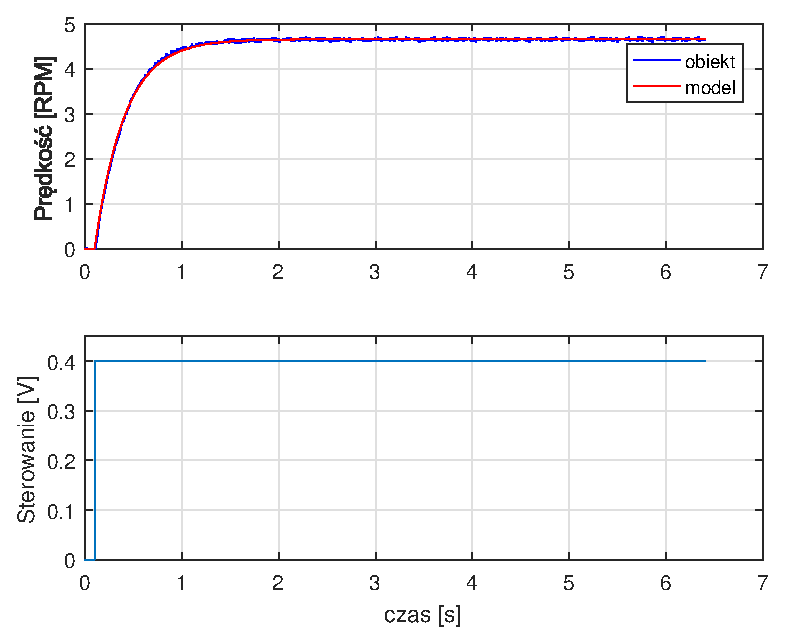
\includegraphics[scale = 1]{fig/Azimuth_iden.eps}
	\caption		
	{Charakterystyka śmigła oś pozioma.}
\end{figure} 
W przypadku osi poziomej model śmigła opisany jest następującą transmitancją:
\begin{equation}\label{key}
G(s) = \frac{K}{Ts + 1} = \frac{11.63}{0.31s + 1}
\end{equation}

\begin{figure}[h!]
	\centering
	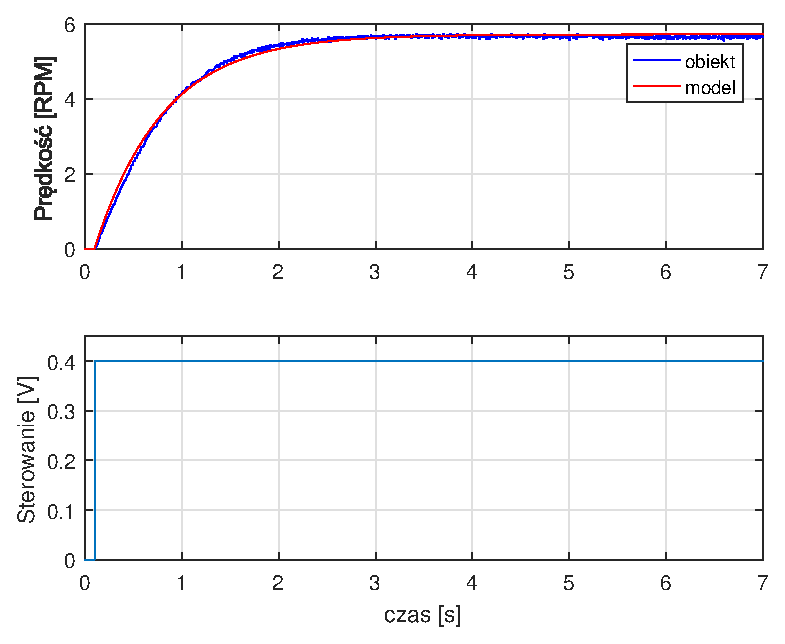
\includegraphics[scale = 1]{fig/Pitch_iden.eps}
	\caption		
	{Charakterystyka śmigła oś pionowa.}
\end{figure} 
Natomiast dla osi pionowej : 
\begin{equation}\label{key}
G(s) = \frac{K}{Ts + 1} = \frac{14.28}{0.71s + 1}
\end{equation}
 
 
\section{Charakterystyka statyczna helikoptera.}

Do wyznaczenia zależności generowanego momentu siły przez śmigło odpowiedzialne za ruch wzdłuż osi pionowej przeprowadzono eksperyment polegający na doczepianiu ciężarków o różnej masie z drugiej strony helikoptera i równoważeniu tak powstałego momentu siły przez odpowiednie dobranie prędkości obrotowej. W tabeli \ref{char_statyczna_tabela} podano otrzymane dane. 
\begin{table}[h]
	\caption{Porównanie poszczególnych regulatorów LQR.}
	\label{char_statyczna_tabela}
	\centering
	
	\begin{tabular}{|c|M{2.5cm}|M{2.5cm}|M{2.5cm}|}
		\hline
		Masa [g]&Prędkość [RPM]&Wsp. PWM [\%]&Moment siły [Nm]\\

		\hline
		0	&	7.1  & 63 & 0\\
		\hline
		15	&  6.3 &  51  & 0.0338\\
		\hline
		30	& 5.2	& 37 &  0.0677\\
		\hline
		45	& 3.75 & 32 &  0.1015\\
		\hline	
		60	& 0	&  0 &  0.1354\\
		\hline
		75	& -5.15	& -33  &   0.1692\\
		\hline
		90	&	-7.05 & -57 &   0.2031\\
		\hline
		105	&	-8.7 & -85 & 0.2369\\
		\hline
	\end{tabular}
\end{table}
Na podstawie zależności momentu siły od prędkości wyznaczono wielomian aproksymujący rzędu trzeciego opisanego zależnością : 
\begin{equation}\label{key}
M(v) = -0.000167v^3 -0.000755 v^2  - 0.0054v + 0.1390
\end{equation}

\begin{figure}[h!]
	\centering
	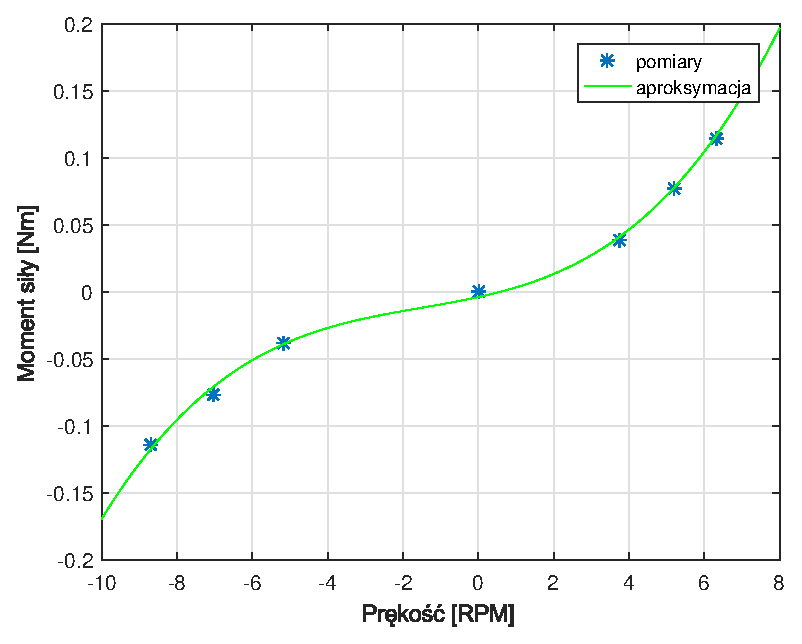
\includegraphics[scale = 1]{fig/char_statyczna.eps}
	\caption		
	{Charakterystyka statyczna śmigła oś pionowa.}
\end{figure} 
